% called by main.tex
%
\chapter{Material y métodos}
\label{ch::metodos}

Este capítulo describe el material (los datos) y los métodos (líneas base, protocolo de
validación y modelos) del trabajo. Se ha organizado en tres bloques: la descripción del
conjunto de datos, los resultados de las líneas base —que contienen la lección central del
trabajo— y la metodología de modelado y entrenamiento.

\section{Descripción del dataset}

\subsection{Sistema de captura multifuente}

Para este trabajo se desarrolló un sistema de captura propio. Por cada sesión de mercado
registra el libro de órdenes de Polymarket, el flujo de operaciones, la metadata del
mercado y un conjunto de referencias externas del mercado de Bitcoin: el mercado al contado
(\emph{spot}), los futuros perpetuos (\emph{perpetual futures}) y un oráculo de precios.
Todas esas fuentes se alinean en el tiempo sobre una malla regular de dos segundos
(Figura~\ref{fig:captura}).

\begin{figure}[h]
\centering
\begin{tikzpicture}[
  node distance=6mm and 14mm,
  src/.style={draw, rounded corners, fill=blue!6, align=center, minimum width=26mm, minimum height=8mm, font=\small},
  proc/.style={draw, rounded corners, fill=orange!12, thick, align=center, minimum width=30mm, minimum height=9mm, font=\small},
  res/.style={draw, rounded corners, fill=green!10, align=center, minimum width=30mm, minimum height=9mm, font=\small},
]
\node[src] (pm) {Polymarket\\(libro + trades)};
\node[src, below=of pm] (spot) {Spot BTC};
\node[src, below=of spot] (perp) {Perp BTC};
\node[src, below=of perp] (orac) {Oráculo};
\node[proc, right=of spot] (align) {Alineación temporal\\malla de 2\,s};
\node[proc, right=of align] (qa) {Control de calidad\\por sesión};
\node[res, right=of qa] (corp) {Corpus\\\texttt{sesión}$\times$\texttt{token}$\times t$};
\draw[-{Latex}] (pm.east) -- (align.west);
\draw[-{Latex}] (spot.east) -- (align.west);
\draw[-{Latex}] (perp.east) -- (align.west);
\draw[-{Latex}] (orac.east) -- (align.west);
\draw[-{Latex}] (align) -- (qa);
\draw[-{Latex}] (qa) -- (corp);
\end{tikzpicture}
\caption{Arquitectura del sistema de captura. Las cuatro fuentes se alinean sobre una malla
de dos segundos, pasan un control de calidad por sesión y forman el corpus.}
\label{fig:captura}
\end{figure}

La elección de la malla de dos segundos no es un detalle accesorio: fija el
\emph{contrato de latencia} con el que después se evalúa. En lugar de interpolar un instante
no observado, las predicciones se miden contra la siguiente fotografía real del mercado, lo
que hace la evaluación conservadora y realista.

\subsection{Controles de calidad por sesión}

Antes de incorporarse al corpus, cada sesión pasa una serie de controles de calidad:
cobertura temporal, continuidad, proporción de datos obsoletos (\emph{stale}), validación
del arranque y detección de huecos severos. La sesión que no supera los umbrales se
descarta. Esta decisión es deliberada: una referencia externa retrasada o incompleta puede
inducir una señal espuria, y se prefiere reducir el tamaño de la muestra antes que
contaminar el entrenamiento con ruido disfrazado de patrón.

\subsection{Composición del corpus}

El corpus principal abarca del 11 al 25 de mayo de 2026 (entrenamiento, validación y test
terminal), con del orden de 2,6 millones de filas \emph{cross-venue}. Como conjunto fuera
de muestra se reservó del 6 al 10 de junio de 2026, capturado con posterioridad a la
congelación del candidato (Sección~\ref{sec:congelacion}). La unidad de observación es la
tupla \texttt{sesión $\times$ token $\times$ instante} sobre la malla de dos segundos. La
Figura~\ref{fig:timeline} resume la partición temporal.

\begin{figure}[h]
\centering
\begin{tikzpicture}[font=\small, >=Latex]
  \draw[-{Latex}] (0,0) -- (13.2,0);
  \foreach \x/\lab in {0/{11 may}, 4.5/{20 may}, 6/{22 may}, 7.8/{25 may}, 10/{6 jun}, 12.6/{10 jun}}
    \draw (\x,0.1) -- (\x,-0.1) node[below, font=\scriptsize] {\lab};
  \draw[line width=4pt, blue!55] (0,0.35) -- (4.5,0.35) node[midway, above, font=\scriptsize, black] {Entrenamiento};
  \draw[line width=4pt, teal!55] (4.5,0.35) -- (6,0.35) node[midway, above, font=\scriptsize, black] {Valid.};
  \draw[line width=4pt, purple!55] (6,0.35) -- (7.8,0.35) node[midway, above, font=\scriptsize, black] {Test};
  \draw[line width=4pt, orange!75] (10,0.35) -- (12.6,0.35) node[midway, above, font=\scriptsize, black] {Fuera de muestra};
  \node[font=\scriptsize, align=center] at (8.9,0.35) {(congelación)};
\end{tikzpicture}
\caption{Partición temporal del corpus. El conjunto fuera de muestra (6--10 jun) se capturó
después de congelar el candidato, lo que convierte su validación en una prueba genuina.}
\label{fig:timeline}
\end{figure}

\subsection{Análisis exploratorio del corpus}

El análisis exploratorio previo deja cuatro observaciones que condicionan todo el diseño
posterior:

\begin{enumerate}[noitemsep]
  \item \textbf{Desequilibrio de clases.} La etiqueta direccional está dominada por la
  clase \textsc{flat} (quietud): a horizonte de 60 segundos, entre el 55 y el 65\,\% de las
  observaciones caen dentro de la banda de quietud. Esto vuelve engañosa la precisión bruta
  —un modelo que prediga siempre \textsc{flat} ya supera el 60\,\%— y obliga a usar
  precisión equilibrada (\emph{balanced accuracy}) y F1 macro.
  \item \textbf{Calidad de los datos.} En los tramos de alta volatilidad, los retardos de
  actualización de las referencias externas abarcan varios ciclos de la malla; tras el
  filtrado, el corpus efectivo es bastante menor que el total capturado, lo que justifica
  una regularización agresiva.
  \item \textbf{Patrón \emph{prestart}.} La ventana inmediatamente anterior a la apertura
  del mercado concentra una densidad atípica de cancelaciones, modificaciones y cruces, lo
  que sugiere reposicionamiento de los participantes y una señal de microestructura
  diferenciada. Esta observación motiva el especialista descrito más adelante.
  \item \textbf{Acoplamiento con Bitcoin.} La correlación entre el precio del contrato y las
  referencias de Bitcoin es clara en ventanas de minutos pero se diluye en ventanas de
  segundos: el arbitraje externo no es instantáneo. Esa separación de escalas justifica
  combinar el libro local con las referencias externas.
\end{enumerate}

\section{Resultados en modelos baseline}

\subsection{Línea base tabular y el impacto de la latencia}

Una línea base tabular sobre el horizonte corto (16 segundos) alcanza una precisión
direccional cercana al 90\,\% y supera la validación temporal por bloques. Evaluada solo
con métricas de clasificación, parece un modelo excelente. El problema aparece al introducir
la entrada retrasada y el coste. La Tabla~\ref{tab:latencia} y la Figura~\ref{fig:latencia}
muestran el rendimiento en el test terminal —el bloque no utilizado para seleccionar la
política— en función de la latencia de entrada, en un escenario conservador con filtro de
\emph{spread}.

\begin{table}[h]
\centering
\caption{Rendimiento en el test terminal bajo distintas latencias (ticks netos).}
\label{tab:latencia}
\begin{tabular}{rrrrr}
\toprule
\textbf{Latencia} & \textbf{Acciones} & \textbf{Acierto UP} & \textbf{Neto medio} & \textbf{Neto total} \\
\midrule
0\,s & 64 & 92,2\,\% & $+6{,}79$ & $+434{,}44$ \\
2\,s & 63 & 39,7\,\% & $-1{,}48$ & $-93{,}48$ \\
4\,s & 66 & 45,5\,\% & $-0{,}74$ & $-48{,}83$ \\
8\,s & 66 & 43,9\,\% & $-0{,}30$ & $-19{,}53$ \\
\bottomrule
\end{tabular}
\end{table}

\begin{figure}[h]
\centering
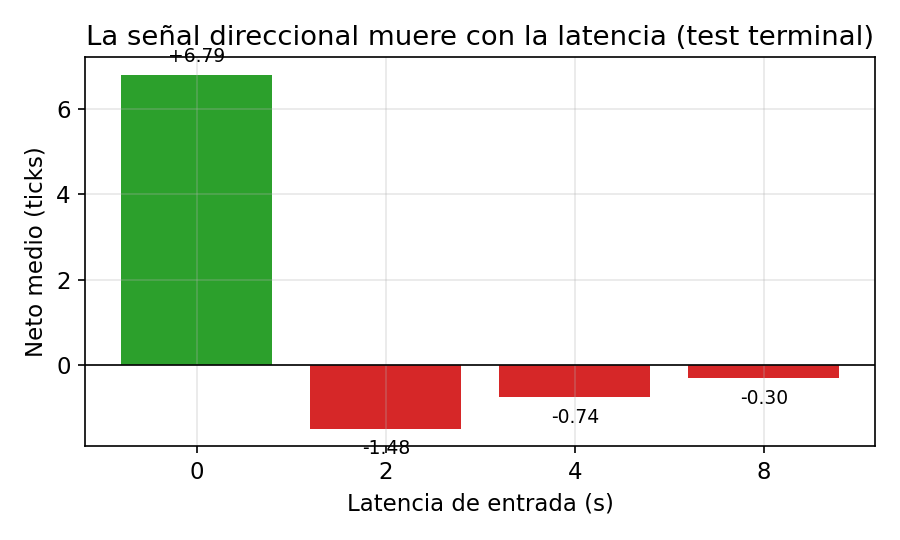
\includegraphics[width=0.7\textwidth]{figures/fig_latencia.png}
\caption{Neto medio en el test terminal frente a la latencia de entrada. La señal a latencia
nula es real como \emph{markout} desde el instante de la señal, pero no sobrevive como
política ejecutable con dos segundos de latencia.}
\label{fig:latencia}
\end{figure}

Este es el resultado que vertebra todo el trabajo: \textbf{acertar la dirección no equivale
a obtener beneficio}. Con una latencia realista de dos segundos, el neto medio del test
terminal cae a $-1{,}48$ ticks. El problema deja de ser de clasificación y pasa a ser de
ejecución; a partir de aquí, todo modelo se evalúa por su política económica bajo coste y
latencia, no por su acierto.

\section{Metodología y entrenamiento}

\subsection{Definición del objetivo}

Para cada instante $t$ se define el retorno futuro del precio medio a un horizonte $H$,
\begin{equation}
\Delta_H(t) = \frac{m_{t+H} - m_t}{m_t},
\end{equation}
donde $m_t$ es el precio medio del contrato. La etiqueta direccional se obtiene con un
umbral $\theta$ que absorbe el \emph{spread}, las comisiones y el ruido:
\begin{equation}
y_t = \begin{cases}
\textsc{up} & \text{si } \Delta_H(t) > \theta,\\[2pt]
\textsc{down} & \text{si } \Delta_H(t) < -\theta,\\[2pt]
\textsc{flat} & \text{en otro caso.}
\end{cases}
\end{equation}
Esta etiqueta ternaria es útil para mirar el arco experimental en su conjunto; el
especialista final, en cambio, usa los dos objetivos económicos que se definen más abajo.
Las características son causales (solo usan información hasta
$t$) y las etiquetas se calculan \emph{a posteriori} de forma trazable, de modo que no
entra información del futuro por las entradas del modelo. Todos los resultados económicos se
expresan en ticks netos, que es la unidad natural del libro; no se traducen a dinero porque
ello exigiría suponer un tamaño de posición y favorecería la sobreafirmación.

\paragraph{Los dos objetivos del especialista.} El modelo final no usa la etiqueta ternaria,
sino dos objetivos complementarios, porque un modelo que debe decidir si entra necesita
saber algo más fino que la dirección: cuánto vale la operación y si el entorno de ejecución
es favorable (Figura~\ref{fig:doscabezas}).

\begin{figure}[h]
\centering
\begin{tikzpicture}[
  node distance=5mm and 12mm, font=\small, >=Latex,
  io/.style={draw, rounded corners, fill=blue!6, align=center, minimum width=30mm, minimum height=9mm},
  head/.style={draw, rounded corners, fill=orange!12, thick, align=center, minimum width=42mm, minimum height=11mm},
  dec/.style={draw, rounded corners, fill=green!10, align=center, minimum width=34mm, minimum height=11mm},
]
\node[io] (x) {36 características\\causales (\emph{no\_clock})};
\node[head, right=of x, yshift=9mm] (reg) {Regresor EV\\\texttt{exec\_net\_cost\_0p25}};
\node[head, right=of x, yshift=-11mm] (clf) {Clasificador salud\\\texttt{healthy\_fill\_proxy}};
\node[dec, right=14mm of $(reg)!0.5!(clf)$] (pol) {Operar si\\EV $>0{,}75$ \emph{y}\\P(salud)$\ge 0{,}50$};
\draw[-{Latex}] (x.east) -- (reg.west);
\draw[-{Latex}] (x.east) -- (clf.west);
\draw[-{Latex}] (reg.east) -- (pol.west);
\draw[-{Latex}] (clf.east) -- (pol.west);
\end{tikzpicture}
\caption{Modelo de dos cabezas. Un regresor predice el valor esperado de la operación y un
clasificador predice si el relleno será ``sano''. La política exige ambas condiciones.}
\label{fig:doscabezas}
\end{figure}

El \textbf{regresor} predice \texttt{exec\_net\_cost\_0p25\_H60}: el neto ejecutado a 60
segundos tras descontar una fracción (0,25) del coste visible de entrada de cada operación.
El \textbf{clasificador} predice \texttt{healthy\_fill\_proxy\_0p25\_H60}: una variable
binaria que vale 1 cuando ese neto es positivo \emph{y} la operación no cae en el peor
cuartil de un grupo de operaciones comparables (mismo bloque temporal, fase, nivel de
\emph{spread}, microprice y momento del perp). La independencia entre ambas cabezas es
deliberada: una operación puede tener alto valor esperado pero baja probabilidad de relleno
sano si el libro está degradado.

\subsection{Validación temporal y prevención de fuga}

La partición respeta siempre el orden del tiempo: el entrenamiento utiliza las sesiones más
antiguas, la validación las posteriores y el test terminal el bloque final. En los
experimentos secuenciales se emplea además un protocolo fuera de pliegue
(\emph{out-of-fold}): cada modelo se entrena solo con días anteriores, las predicciones que
consume una segunda etapa son siempre fuera de muestra, y la política de decisión se
selecciona sin observar el test terminal. Esta disciplina contra la fuga temporal es la
salvaguarda frente a resultados ilusorios~\cite{lopezdeprado2018,gu2020empirical}.

\subsection{Modelo de costes y latencia}

La latencia no se supone, se mide. En una prueba controlada del ciclo de orden de
Polymarket, el tiempo entre observar la oportunidad y confirmar el emparejamiento fue de
unos 0,43 segundos en el percentil 95 de la muestra válida. Aun así, por prudencia se
trabaja con cifras peores: una latencia conceptual de un segundo y una latencia observable
en los datos de dos segundos (la malla de captura). El coste de ejecución no se fija como un
número plano de ticks, sino como una fracción del coste visible de entrada de cada
operación: la mitad de ese coste como referencia, un cuarto como contraste optimista y el
coste completo como prueba de estrés. Modelar el coste relativo al libro de cada instante es
más fiel que asumir un coste fijo e igual para todas las operaciones. Formalmente, el neto
ejecutado a horizonte $H$ con un factor de coste $c \in \{0,\ 0{,}25,\ 0{,}5,\ 1\}$ es
\begin{equation}
\text{net}_c(t) = \big(\Delta^{\text{ticks}}_H(t) - b\big) - c \cdot \kappa_t,
\label{eq:coste}
\end{equation}
donde $\Delta^{\text{ticks}}_H(t)$ es el \emph{markout} en ticks desde la entrada (a dos
segundos del instante de señal) hasta el horizonte, $b$ es un \emph{buffer} fijo y $\kappa_t$
es el coste visible de entrada de esa operación. Nótese que, por construcción, un factor de
coste mayor produce un neto menor sobre la misma operación; por eso el resultado al coste de
referencia ($c=0{,}5$) es siempre inferior al optimista ($c=0{,}25$) y superior al de estrés
($c=1$).

\subsection{Métricas de evaluación}

La elección de métricas es deliberada y responde a las características del problema. Para la
fase de clasificación no se reporta la precisión bruta (\emph{accuracy}), porque el dominio
de la clase \textsc{flat} la vuelve engañosa; en su lugar se usan la \textbf{precisión
equilibrada} (\emph{balanced accuracy}) y la \textbf{F1 macro}, que promedian por clase y no
premian al modelo que siempre predice quietud. Para medir la capacidad de \emph{ordenar} las
oportunidades se emplea el \textbf{AUC} (área bajo la curva ROC), independiente del umbral.

Ahora bien, la métrica que decide es económica, no de clasificación: el \textbf{neto medio
por operación} bajo el modelo de costes de la ecuación~\eqref{eq:coste}. A su alrededor se
reportan siempre cuatro elementos de soporte e incertidumbre: (i) el \textbf{número de
operaciones y de días}, porque un neto sin soporte no es interpretable; (ii) un
\textbf{intervalo de confianza \emph{bootstrap}} (5\,000 remuestreos, semilla fija); (iii) la
\textbf{probabilidad de neto positivo} estimada sobre esa misma distribución; y (iv) el
\textbf{drawdown máximo} y el número de \textbf{días positivos}, como medidas de estabilidad.
Esta batería evita confundir una señal estadística con una estrategia viable.

\subsection{La escalera de modelos}

Los modelos se evalúan en una progresión incremental, de menor a mayor complejidad,
exigiendo en cada salto que la complejidad añadida se justifique con evidencia de mejora
bajo el mismo protocolo de costes y validación (Figura~\ref{fig:escalera}).

\begin{figure}[h]
\centering
\begin{tikzpicture}[
  node distance=4mm, font=\small, >=Latex,
  rung/.style={draw, rounded corners, align=center, minimum width=0.84\textwidth, minimum height=8mm, inner sep=3pt},
]
\node[rung, fill=blue!6] (s1) {Línea base tabular H16 (acierto $\sim$90\,\%, pero muere con latencia)};
\node[rung, fill=blue!6, below=of s1] (s2) {Modelos sensibles a la latencia (AUC 0,79; política negativa)};
\node[rung, fill=blue!8, below=of s2] (s3) {Secuencias y libro: GRU, Conv1D (\emph{BookEncoder}), fusión, TCN (representación sí, política no)};
\node[rung, fill=orange!10, below=of s3] (s4) {Corrección del \emph{score} de selección adversa; selección de horizonte (H60)};
\node[rung, fill=green!12, thick, below=of s4] (s5) {Especialista \emph{prestart} H60 (HGB de dos cabezas) + filtro de volatilidad};
\draw[-{Latex}] (s1)--(s2); \draw[-{Latex}] (s2)--(s3); \draw[-{Latex}] (s3)--(s4); \draw[-{Latex}] (s4)--(s5);
\end{tikzpicture}
\caption{La escalera de modelos. Cada paso debe superar al anterior bajo el mismo protocolo;
si no lo hace, se descarta.}
\label{fig:escalera}
\end{figure}

Los \textbf{modelos sensibles a la latencia} incorporan la latencia en el etiquetado y la
selección; uno de ellos alcanza un AUC de test de 0,79 y, pese a ello, su política económica
sigue siendo negativa. Sobre el \textbf{libro de órdenes} se construyen secuencias de ocho
pasos y un tensor de los diez primeros niveles, y se evalúan una red recurrente (GRU, capa
oculta de dimensión 56), un codificador convolucional del libro (\emph{BookEncoder}, dos
capas Conv1D con \emph{pooling} medio y máximo, inspirado en
DeepLOB~\cite{zhang2019deeplob,tsantekidis2017}), una fusión de ambos y una red convolucional
temporal (TCN) para el régimen de volatilidad. El \emph{BookEncoder} resume cada fotografía
del libro con dos convoluciones unidimensionales sobre la dimensión de niveles y un
\emph{pooling} dual (medio y máximo):
\begin{equation}
\mathbf{h} = \big[\operatorname{mean}_\tau\, \phi(\mathbf{B}_\tau)\ \|\ \operatorname{max}_\tau\, \phi(\mathbf{B}_\tau)\big],
\quad
\phi = \text{ReLU}\!\circ\!\text{Conv1d}\!\circ\!\text{Dropout}\!\circ\!\text{ReLU}\!\circ\!\text{Conv1d},
\end{equation}
donde $\mathbf{B}_\tau$ es el libro en el paso $\tau$ de la secuencia y $\|$ denota
concatenación. El \emph{pooling} máximo capta los picos de profundidad, a menudo más
informativos que la media en mercados poco líquidos. Estas arquitecturas aprenden
representación, pero no producen una política estable con un horizonte de entrenamiento de
unas dos semanas (unos 5\,800 ejemplos): el aprendizaje profundo se aparca a la espera de
más datos.

Durante la auditoría se detectó y corrigió un error de interpretación en el \emph{score} de
selección adversa (su orientación correcta es $1 - P(\text{adverso})$), lo que ilustra que
una métrica positiva no basta sin auditar su significado económico. Por último, al comparar
horizontes (Tabla~\ref{tab:horizonte}), solo H60 conserva señal; H120 y H240 colapsan, por
lo que H60 queda como único candidato.

\begin{table}[h]
\centering
\caption{Selección de horizonte (ticks netos \emph{proxy}). Solo H60 conserva señal.}
\label{tab:horizonte}
\begin{tabular}{lrr}
\toprule
\textbf{Métrica} & \textbf{H60} & \textbf{H120} \\
\midrule
AUC test                       & $0{,}565$ & $0{,}495$ \\
Top 35\,\% test, coste $0{,}5$ & $+0{,}426$ & $-1{,}117$ \\
Top 35\,\% test, coste $1{,}0$ & $+0{,}058$ & $-1{,}491$ \\
\bottomrule
\end{tabular}
\end{table}

\subsection{Especialista \emph{prestart} H60}

El candidato final es un especialista para la ventana \emph{prestart}: un modelo de
\emph{gradient boosting} sobre histogramas (HistGradientBoosting) con las dos cabezas
descritas, entrenado sobre 36 características sin variables de reloj (para evitar atajos
temporales triviales). La señal se restringe a la ventana de $-60$ a $-45$ segundos respecto
a la apertura, con libro saludable y coste visible acotado (Figura~\ref{fig:prestart}).

\begin{figure}[h]
\centering
\begin{tikzpicture}[font=\small, >=Latex]
  \draw[-{Latex}] (-0.5,0) -- (10.8,0) node[right, font=\scriptsize] {tiempo};
  \fill[orange!25] (1,-0.18) rectangle (3.5,0.18);
  \node[font=\scriptsize, align=center] at (2.25,0.6) {ventana \emph{prestart}\\$-60$ a $-45$\,s};
  \draw[dashed] (8.5,-0.7) -- (8.5,0.9);
  \node[font=\scriptsize, align=center] at (8.5,1.1) {apertura\\del mercado};
  \foreach \x/\lab in {1/{$-60$\,s}, 3.5/{$-45$\,s}, 8.5/{$0$}}
    \draw (\x,0.12) -- (\x,-0.12) node[below, font=\scriptsize] {\lab};
  \node[font=\scriptsize, align=center, gray] at (5.9,-0.6) {(resto del \emph{prestart}: no se opera)};
\end{tikzpicture}
\caption{La ventana \emph{prestart} del especialista: solo se opera entre $-60$ y $-45$
segundos respecto a la apertura del mercado, donde el análisis exploratorio detectó una
densidad atípica de actividad del libro.}
\label{fig:prestart}
\end{figure} Ambas cabezas comparten una
configuración de regularización agresiva (tasa de aprendizaje 0,045, hasta 220 iteraciones
con parada anticipada, máximo de 15 hojas por árbol, mínimo de 120 muestras por hoja y
regularización L2 de 0,10), necesaria porque el bloque de entrenamiento del especialista
tiene del orden de mil observaciones útiles. La política congelada opera cuando el valor
esperado predicho supera 0,75 y la probabilidad de salud no baja de 0,50; ambos umbrales se
seleccionaron sobre el conjunto de validación, nunca sobre el test terminal.

\subsection{Filtro de volatilidad}

Al preparar la validación fuera de muestra se observó un cambio de régimen: la fracción de
sesiones de alta volatilidad pasó de un 18--22\,\% en entrenamiento a alrededor del 58\,\% en
el conjunto fuera de muestra (véase la Figura~\ref{fig:regimen} del
Capítulo~\ref{ch::resultados}). Como el modelo aprendió en un régimen de baja volatilidad y
sus predicciones en alta volatilidad no son fiables bajo la distribución desplazada, se
introduce un filtro simple que solo habilita la operativa cuando la volatilidad realizada a
cinco segundos no supera el umbral 0,6657, correspondiente al percentil 80 de la volatilidad
de entrenamiento (un umbral fijado con los datos antiguos, no ajustado a los nuevos).

\subsection{Protocolo de congelación}
\label{sec:congelacion}

El candidato final —modelo, conjunto de características y umbrales de política— se congeló
antes de observar el conjunto fuera de muestra del 6 al 10 de junio. Esta decisión convierte
la validación posterior en una prueba fuera de muestra genuina, y previene el sobreajuste por
selección múltiple~\cite{bailey2014deflated}. Una vez fijada, la política no se reajusta para
mejorar los resultados.
